\hypersetup{linkcolor=purple}
\definecolor{dkgreen}{rgb}{0,0.6,0}
\definecolor{gray}{rgb}{0.5,0.5,0.5}
\definecolor{mauve}{rgb}{0.58,0,0.82}
\lstdefinelanguage{LLVM}{
  morekeywords={define,declare,void,i1,i8,i16,i32,i64,float,double,type,label,align,ret,add,sub,mul,icmp,eq,ne,ugt,ult,slt,sge,br,load,store,call,nuw,nsw},
  sensitive=true,
  morecomment=[l]{;},
  morestring=[b]",
}
\lstset{
  language=LLVM,
  basicstyle=\ttfamily\small,
  keywordstyle=\color{blue}\bfseries,
  commentstyle=\color{gray},
  stringstyle=\color{red},
  numbers=left,
  numberstyle=\tiny\color{gray},
  breaklines=true,
  showstringspaces=false,
}
\chapter{Introduction}

Compilers are complex pieces of software that transform source code written in high-level programming languages into machine code tailored for specific hardware architectures. During compilation, various optimizations are applied to improve code performance on the target platform. Today, production compilers are typically large-scale, open-source projects e.g. the LLVM compiler project, consisting of hundreds of thousands of lines of code contributed by an active developer community. Optimization passes in compilers range from simple local transformations (Fig. \ref{fig:intro_constant_folding}) to sophisticated global analyses, including interprocedural optimizations across function calls and loop transformations. These optimizations are typically driven by performance heuristics and are implicitly assumed to preserve the program semantics. However, they do not exhibit formal guarantees that they preserve program behavior in all cases. 

\begin{figure}[ht]
\centering
\begin{minipage}{0.45\textwidth}
\begin{lstlisting}[language=LLVM]

define i32 @add_unoptimized() {
entry:
  %a = add i32 2, 3
  ret i32 %a
}
\end{lstlisting}
\end{minipage}
\hspace{0.05\textwidth}
\begin{minipage}{0.45\textwidth}
\begin{lstlisting}[language=LLVM]
define i32 @add_optimized() {
entry:
  ret i32 5
}
\end{lstlisting}
\end{minipage}
\caption{Example of a compiler optimization via constant folding. The addition gets replaced with the constant return value.}
\label{fig:intro_constant_folding}
\end{figure}

Although compiler optimizations traditionally aim to maximize runtime performance, they can introduce miscompilation bugs. In such cases, the compiled code no longer preserves the intended semantics of the source program, causing unexpected behavior at runtime.

Compilation bugs arise from mistakes in the compiler’s source code or from the absence of formal semantics for the source and target languages. Formal semantics define the meaning of each language construct e.g. an instruction in a precise, mathematical manner (Fig. \ref{fig:intro_semantics}). If the semantics of a language are not clearly formalized, it can lead to ambiguities about what constitutes correct behavior. This ambiguity effectively grants compiler developers implicit freedom to interpret the semantics of their optimizations, leading to inconsistencies in determining which optimizations are correct. For example, a programming language should define the behavior of integer overflow, otherwise, compilers may handle it differently, leading to inconsistent results.

\begin{figure}
\begin{minipage}{\textwidth}
\begin{lstlisting}
def execute_SHIFTIOP (shamt : BitVec 6) (op : sop) (rs1_val : BitVec 64) : BitVec 64 := match op with
      | sop.RISCV_SLLI => (shift_bits_left rs1_val shamt)
      | sop.RISCV_SRLI => (shift_bits_right rs1_val shamt)
      | sop.RISCV_SRAI => (shift_bits_right_arith (rs1_val) shamt)
\end{lstlisting}
\end{minipage}
\caption{
Formalization of the RISC-V 64-bit shift-immediate instructions. Each instruction is mapped to its corresponding bit-level operation, providing a precise, unambiguous definition.}
\label{fig:intro_semantics}
\end{figure}

In order to avoid these issues, research projects have developed fully verified compilers that provide correctness guarantees for their code. A prominent example is CompCert \cite{CompCertPaper}, the fully verified compiler for the C programming language, which ensures that the semantics of the source program are preserved during compilation. Verified compilers like CompCert demonstrate the possibility of building trustworthy compiler pipelines but their extra proof burden makes them challenging to develop and evolve. 

Fully formally verified compilers typically support only a limited subset of the optimizations and analysis available in their non-verified counterparts. "Adding optimizations is limited by the effort required to verify them", as stated in a CompCert related publication \cite{Mullen2016}. CompCert includes 8 optimization passes and does not support loop transformations e.g merging two adjacent loops with the same bounds into one, whereas other compilers like LLVM provides over 20 loop-specific optimization and analysis passes alone.\cite{compcert_web} 

%[https://www.absint.com/factsheets/factsheet
%\_compcert\_c\_web.pdf]
%[based on -opt -print-passes]
%to pass 
Verified compilation projects do exist, but they often struggle to keep up with the rapid pace of modern compiler development. This is largely due to the need for manual proofs, which not only slows down development but also leads to rigid designs that make adding new optimizations labor intensive. This high proof burden therefore discourages flexibility and new optimizations. This is in contrast to mainstream unverified compilers, where developers contribute new patches daily.

%Moreover, they are typically developed as standalone, complex projects targeting a narrow niche audience e.g. CompCert. This %disconnects them from compiler engineers, who rely on flexible and extensible infrastructure in their day-to-day work in %compiler design.

 LLVM (Low-Level Virtual Machine) is a widely used open-source compiler infrastructure framework that serves as the middle and backend of compilers for modern programming languages, including Rust and Lean. It's strengths are its modular and extensible design centered around it's intermediate representation (IR) \cite{llvm_ref}.(Section XY)

A compiler IR such as LLVM IR for LLVM, enables language-agnostic optimization by abstracting away the specific features of source languages. In LLVM, programs are first translated into the uniform, high-level, assembly-like LLVM IR, which is then optimized in an iterative manner by applying passes (Fig. \ref{fig:intro_llvm}). These passes are either predefined within LLVM or supplied by the user. By implementing a frontend that lowers source code to LLVM IR, compiler developers can immediately take advantage of LLVM's powerful infrastructure, which makes LLVM attractive for building new compilers.
\cite{}
\begin{figure}[htbp]
  \centering
  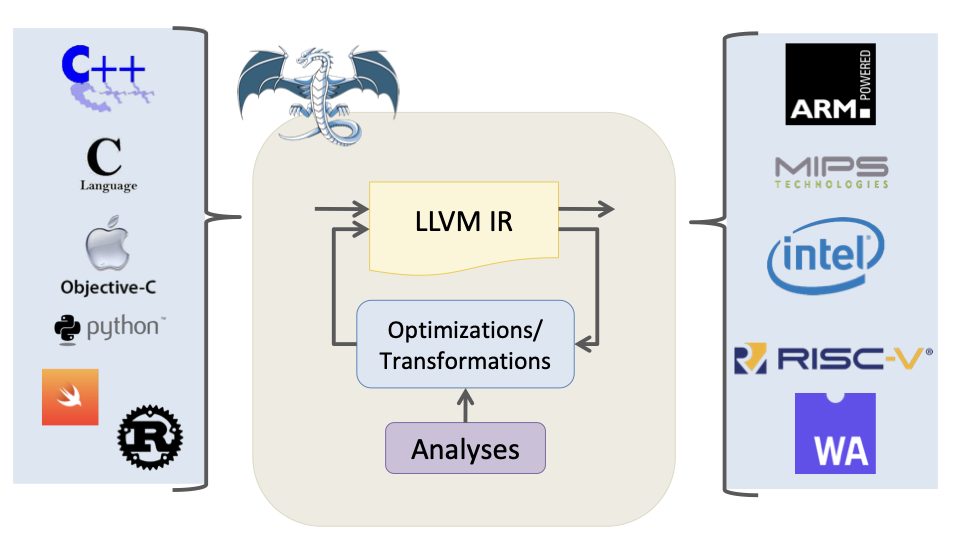
\includegraphics[scale=0.4]{thesis/llvm.png}
  \caption{The LLVM compiler infrastructure centered around LLVM IR}
  \label{fig:intro_llvm}
\end{figure}

Due to the current complexity and size of LLVM, full verification of the entire compilation toolchain is unlikely. At the same time, developers continuously discover bugs in LLVM. A bug in LLVM can affect any language whose compiler relies on it and thereby compromise the correctness of compiled programs across multiple languages.
For example, LLVM is used in the compilation of Lean, which serves not only as a programming language but as a theorem prover\cite {}.(Chaptre XY) In Lean, the compiler is part of the trusted code base and used in proof techniques where a computation is executed its result reused within a proof. The soundness of these proofs therefore hinge on the trustworthiness of the compiler.  Similarly, the Rust compiler uses LLVM in its standard compilation pipeline [\cite{Rustlantis}. While Rust's type system focus on ensuring safety at the Rust language level, once compiled, the correctness of the final machine code relies entirely on the reliability of the LLVM toolchain. This makes compilers and especially the LLVM ecosystem an interesting and important target for the application of formal methods and compiler verification.

\begin{figure}[htbp]
  \centering
  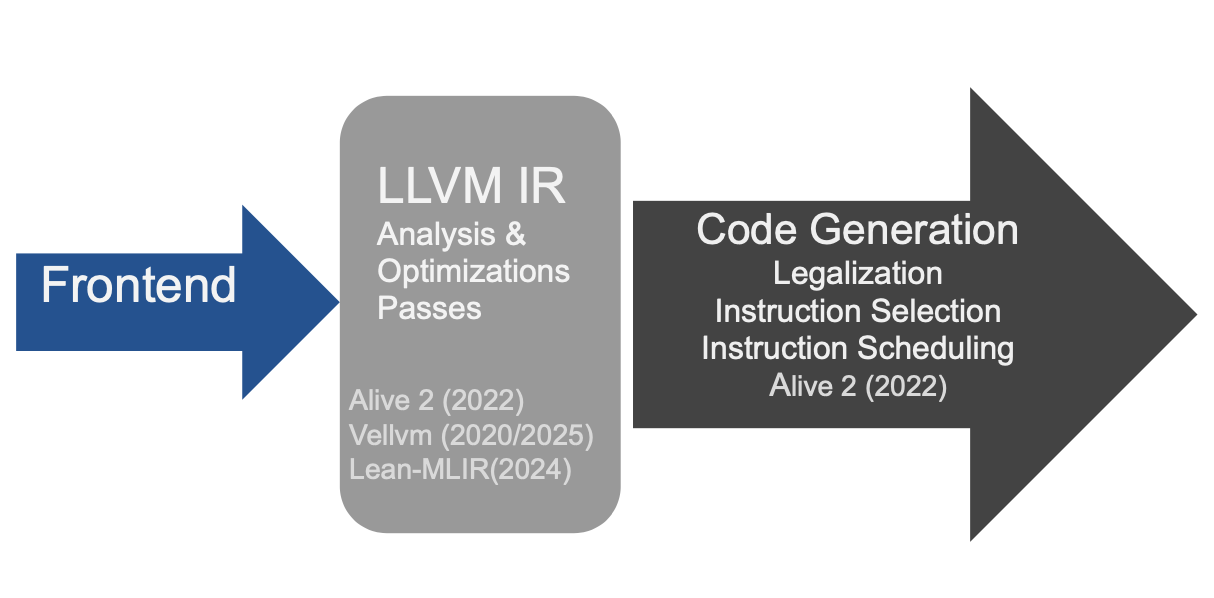
\includegraphics[scale=0.35]{thesis/verification_efforts_intro.png}
  \caption{Verification efforts within the LLVM ecosystem}
  \label{fig:your-label}
\end{figure}

At the time of this thesis, several verification efforts target the LLVM ecosystem, particularly around LLVM IR. For example, the Alive2 project verifies optimizations used in LLVM’s InstCombine pass, a peephole optimization pass for LLVM IR [Quote]. Peephole optimizations are small, local transformations that replace short sequences of instructions with semantically equivalent but more efficient alternatives [Quote: Peephole paper]. The size of LLVM's peephole rewriter which accounts  for  10\% of the IR-transforming codebase, emphasizes its significance within the LLVM toolchain. \cite{Bhat2024Verify}
Besides the higher-level stack around LLVM IR, only few efforts target the lower levels of the LLVM compiler toolchain, such as instruction selection. Yet these lower-level components are known as one of the most error-prone parts of a compiler. A common feature verification efforts in general is their reliance on SMT solvers for proving correctness. While SMT solvers enable automated verification, correctness now hinges not on the compiler’s source code, but on the large codebase of the solver itself. The large codebase of SMT solvers has historically been found to contain many bugs \cite{Nuno2021Alive2}

\textbf{Our approach:} To counteract these limitations, we propose a verified instruction selection pipeline and an RISC-V assembly peephole optimization pass for LLVM IR, implemented within an interactive theorem prover. Our approach resolves various problems mentioned above. Firstly, we model instruction selection as a collection of locally verified rewrite rules. This allows new patterns and therefore new instruction lowerings to be added with minimal effort and avoids the need to modify core verification infrastructure. Furthermore, our verification setup is designed to take advantage of proof automation for reasoning about the semantics of compiler IRs and low-level assembly instructions. We design both our instruction selection and optimization passes to allow existing automation tools to handle the majority of proof obligations automatically. This enables developers to focus on writing new patterns, which are then automatically verified, minimizing the proof burden typically encountered in verified compiler projects. By implementing an instruction selection pass and an RISC-V optimization pass, our work also redirects attention to the compiler backend. Compiler backends, especially within the LLVM ecosystem, have received little attention in formal verification efforts. We choose LLVM IR as our source language for our instruction selection not only because LLVM is known for its IR, but also because it serves as the foundation for many of today's compilers. 

We choose the Lean theorem prover as our verification infrastructure due to its minimal trusted codebase and strong support for proof automation. This small trusted base ensures that the correctness of our verified components depends only on a well-scoped codebase, unlike approaches that rely on large SMT solvers. Lean also offers powerful automation capabilities, particularly for bit-vector reasoning. This is crucial for our work, as the semantics of low-level assembly instructions are typically formalized using bit-vector operations.

Additionally, a formalization of the RISC-V instruction set architecture (ISA) exists in Lean. By selecting RISC-V as our target architecture, we are able to derive semantics directly from these mechanized models, which are officially accepted by RISC-V International. This provides strong correctness guarantees for our semantics, in contrast to approaches where ISA semantics are manually derived from online documentations.

Both Lean and its tooling are designed with scalability in mind, which is crucial for supporting large and evolving compiler verification efforts. Furthermore, the ongoing Lean-MLIR project provides a framework for modeling compiler intermediate representations (IRs) within Lean, which provides the starting point of our work. Lean-MLIR explicitly allows to model MLIR dialects in Lean.
MLIR, part of the LLVM ecosystem, is a compiler infrastructure that supports multiple domain-specific, SSA-based intermediate representations (dialects) within a unified framework. In Static Single Assignment (SSA) form, each variable is assigned exactly once, which simplifies program analysis and transformation. MLIR allows different parts of a program to be represented in different dialects, enabling multiple levels of abstraction within a single program. This flexibility allows optimizations to be applied at the level where the most relevant semantic information is available. Because an MLIR program can contain multiple dialects simultaneously, it is often referred to as a hybrid IR.
\begin{figure}[ht]
\centering
\begin{lstlisting}[language=LLVM, basicstyle=\ttfamily\small]
module {
  func.func @simple_add(%arg0: i32, %arg1: i32) -> i32 {
    %sum = arith.addi %arg0, %arg1 : i32
    return %sum : i32
  }
}

\end{lstlisting}
\caption{ MLIR code using the \texttt{arith}, \texttt{func},  and \texttt{built.in} dialects to perform integer addition. The \texttt{arith} dialect holds integer mathematical operations, the \texttt{func} dialect contains function abstractions. The \texttt{built.in} dialect contains standart operations used across many domains.}
\label{fig:mlir-addition}
\end{figure}
%maybe delte it 
Complementary to LeanMLIR efforts such as the development of a verified floating-point library further reinforce our choice of Lean, as these components are essential in future work on building a complete verified compiler backend.

Currently our instruction selection pipeline lowers LLVM IR—under specific constraints on the input program—into a RISC-V assembly dialect targeting a 64-bit architecture. If the source program conforms to the supported fragment of LLVM IR and our pass succeeds, the generated assembly code is guaranteed to exhibit behavior equivalent to that of the original LLVM IR program. We build on the existing LLVM IR dialect in Lean-MLIR and implement a custom RISC-V dialect, expressing the core of our instruction selection as a lowering transformation between these two dialects. To reason about the correctness of our instruction selection, we rely on precise formal semantics for both the source and target languages. 

In addition, we introduce semantics-preserving assembly-level optimizations that eliminate potential inefficiencies introduced during instruction selection. This ensures not only correctness, but also performance improvements at the machine code level. To implement our verified peephole optimization pass, we analyze and adapt patterns used in compiler passes such as InstCombine and DagCombine, which are optimization passes within LLVM. [NOTE:That would be my plan]
To visualize the transformed code, we provide a command-line interface for our instruction selection pass, inspired by the LLVM optimizer. 

For verification, we leverage Lean’s novel and comprehensive bit-vector library, along with bv\_decide, the first fully verified SMT solver embedded in a theorem prover. Bv\_decide provides automation for fixed-width bit-vector expressions, which we use to automatically prove the correctness of our rewrite rules.

\textbf{Contributions}

Explicitly, we contribute the following:

\begin{itemize}
\item {Implement a RISCV-V dialect in Lean-MLIR which models RISC-V assembly operations in Lean. The RISC-V dialect in Lean is given with proofs that the dialect exactly implement the semantics as specified by the Sail RISC-V model for 64-bit address space processors.}

\item {Implement a hybrid LLVM and RISC-V dialect in Lean-MLIR, enabling instruction lowerings as rewrite rules within the dialect, including cast conversions analogous to those in MLIR.}

\item {Design and implement a verified instruction selection pass from the LLVM IR dialect (restricted to the pure arithmetic fragment) to a RISC-V SSA-style assembly dialect, using instruction selection patterns extracted from LLVM.}

\item {Implement a RISC-V peephole optimization pass that includes XY\% of the optimizations performed by the LLVM backends.}

\item {Optimizer command line tool \textit{"opt"} for Lean, that processes LLVM IR files and allows to apply the instruction lowering pass and optimization passes by providing the corresponding flag.
[Note: Also, it doesnt work yet because the input is not LLVM IR files but only regions in LLVM IR dialect style and not even all of the syntax is supported yet. I claim the previous opt tool used wrong MLIR syntax].}

\item {Implement register allocation for the RISC-V SSA-style IR to obtain RISCV-V machine code.
[Note: Lie, not done yet but is part of the vision]}

\item {Assembly Printer that outputs resulting RISC-V machine code.
[note: Lie]}

\item {Lemmas and tactics in Lean that allow to automatically verify new rewrites in Lean}

\end{itemize}

As noted throughout this thesis, due to time constraints and the ongoing development of Lean-MLIR, our work includes a few limitations that we plan to address in the future. However, we believe these do not affect the overall approach we have followed. For example, we focused only on a pure fragment of LLVM IR without side effects. Given the continued progress in Lean-MLIR, we are confident that extending our approach to handle side effects will be feasible in future work.

All code and proofs developed in this thesis have been upstreamed to the Lean-MLIR project and are publicly available.
